\chapter{Results and Discussion}

\section{Experimental Results}

This chapter reports the classification results obtained from high frequency partial discharge (PD) signals acquired from medium voltage overhead lines. Two optimization regimes are compared in terms of their selected feature sets and the resulting classification performance: a Featurewiz based selection track and an MLJAR track. Model performance is presented using Accuracy, Precision, Recall, F1 score, and ROC AUC, with results summarized in the tables and figures that follow.


\section{Comparison of Feature Selection Outcomes}

The first set of results compares the features retained by the two optimization regimes. Table \ref{tab:fs_comparison_outcomes} lists features that were jointly selected, providing a direct view of the overlap between the Featurewiz and MLJAR selections. The shared set spans time domain statistics (for example, rms, skewness, kurtosis, and crest\_factor), frequency domain descriptors (for example, fft\_mean, fft\_max, stft\_mean, stft\_max, and spectral\_entropy), PRPD pattern measures (for example, prpd\_polarity\_ratio and multiple quadrant based differences), and complexity measures (for example, fractal\_dimension and entropy combinations). The prevalence of both original descriptors and interaction terms among the jointly selected features indicates that both regimes consistently retained information reflecting amplitude characteristics, spectral content, phase resolved distribution structure, and signal complexity.

\begin{table}[H]
    \centering
    \caption{Comprehensive Comparison of Feature Selection Outcomes Across FeatureWiz and MLJAR Methods}
    \label{tab:fs_comparison_outcomes}
    \footnotesize
    \resizebox{\textwidth}{!}{%
    \begin{tabular}{|l|l|l|c|c|p{4cm}|}
    \hline
    \textbf{Category} & \textbf{Feature Name} & \textbf{Feature Type} & \textbf{Featurewiz} & \textbf{MLJAR} & \textbf{Reason for Joint Selection} \\
    \hline
    Time Domain & rms & Original & Yes & Yes & Strong amplitude indicator of discharge intensity \\
    \hline
    Time Domain & skewness & Original & Yes & Yes & Captures signal asymmetry \\
    \hline
    Time Domain & kurtosis & Original & Yes & Yes & Sensitive to impulsive transient behavior \\
    \hline
    Time Domain & crest\_factor & Original & Yes & Yes & Highlights peak amplitudes relative to RMS \\
    \hline
    Time Domain & rms\_abs\_diff\_variance & Interaction & Yes & Yes & Measures variation in energy fluctuations \\
    \hline
    Time Domain & kurtosis\_minus\_crest\_factor & Interaction & Yes & Yes & Combines peakiness and impulsiveness metrics \\
    \hline
    Frequency Domain & fft\_mean & Original & Yes & Yes & Average spectral energy across frequencies \\
    \hline
    Frequency Domain & fft\_max & Original & Yes & Yes & Captures dominant spectral bursts \\
    \hline
    Frequency Domain & stft\_mean & Original & Yes & Yes & Represents time-localized spectral average \\
    \hline
    Frequency Domain & stft\_max & Original & Yes & Yes & Represents localized time-frequency energy peaks \\
    \hline
    Frequency Domain & spectral\_entropy & Original & Yes & Yes & Measures spectral complexity or disorder \\
    \hline
    Frequency Domain & fft\_mean\_div\_stft\_mean & Interaction & Yes & Yes & Ratio linking global vs. local spectral energy \\
    \hline
    PRPD Pattern & prpd\_polarity\_ratio & Original & Yes & Yes & Captures asymmetry between positive and negative discharges \\
    \hline
    PRPD Pattern & prpd\_q1\_mean\_minus\_prpd\_q2\_mean & Interaction & Yes & Yes & Quadrant difference reflecting discharge pattern shifts \\
    \hline
    PRPD Pattern & prpd\_q1\_mean\_minus\_prpd\_q3\_mean & Interaction & Yes & Yes & Highlights mid-cycle amplitude differences \\
    \hline
    PRPD Pattern & prpd\_q1\_mean\_minus\_prpd\_q4\_mean & Interaction & Yes & Yes & Captures full-cycle asymmetry \\
    \hline
    PRPD Pattern & prpd\_q2\_mean\_minus\_prpd\_q3\_mean & Interaction & Yes & Yes & Quadrant comparison for pattern variation \\
    \hline
    PRPD Pattern & prpd\_q2\_mean\_minus\_prpd\_q4\_mean & Interaction & Yes & Yes & Highlights mid-to-late cycle differences \\
    \hline
    PRPD Pattern & prpd\_q3\_mean\_minus\_prpd\_q4\_mean & Interaction & Yes & Yes & Detects late-cycle discharge shifts \\
    \hline
    PRPD Pattern & prpd\_q1\_mean\_abs\_diff\_prpd\_q2\_mean & Interaction & Yes & Yes & Absolute difference to quantify pattern change magnitude \\
    \hline
    PRPD Pattern & prpd\_q1\_mean\_abs\_diff\_prpd\_q3\_mean & Interaction & Yes & Yes & Measures deviation between quadrants \\
    \hline
    PRPD Pattern & prpd\_q1\_mean\_abs\_diff\_prpd\_q4\_mean & Interaction & Yes & Yes & Captures maximum cycle asymmetry \\
    \hline
    PRPD Pattern & prpd\_q2\_mean\_abs\_diff\_prpd\_q3\_mean & Interaction & Yes & Yes & Reflects mid-cycle discharge differences \\
    \hline
    PRPD Pattern & prpd\_q2\_mean\_abs\_diff\_prpd\_q4\_mean & Interaction & Yes & Yes & Late-cycle pattern deviation \\
    \hline
    PRPD Pattern & prpd\_q3\_mean\_abs\_diff\_prpd\_q4\_mean & Interaction & Yes & Yes & Detects end-of-cycle pattern changes \\
    \hline
    PRPD Pattern & skewness\_abs\_diff\_prpd\_q1\_density & Interaction & Yes & Yes & Combines shape and distribution variation \\
    \hline
    PRPD Pattern & rms\_div\_skewness & Interaction & Yes & Yes & Links amplitude with asymmetry \\
    \hline
    Complexity \& Entropy & fractal\_dimension & Original & Yes & Yes & Captures signal self-similarity and complexity \\
    \hline
    Complexity \& Entropy & shannon\_entropy\_plus\_spectral\_entropy & Interaction & Yes & Yes & Measures combined randomness in time and frequency \\
    \hline
    Complexity \& Entropy & stft\_max\_abs\_diff\_shannon\_entropy & Interaction & Yes & Yes & Quantifies peak-time spectral irregularity \\
    \hline
    \end{tabular}%
    }
\end{table}

Overall, the overlap in Table \ref{tab:fs_comparison_outcomes} shows that both optimization regimes converged on a common set of informative descriptors across multiple feature categories. In addition to shared original features, the jointly selected interaction terms largely reflect ratios, differences, and absolute differences that relate global and localized spectral summaries and quantify contrasts between PRPD quadrants.

\subsection{Comparative Analysis of Feature Selection Tracks}

The feature selection outcomes are summarized as two tracks. Track 4B corresponds to the Featurewiz selection, resulting in 187 retained features, whereas Track 4C corresponds to the MLJAR feature set, comprising 925 features. Table \ref{tab:feature_tracks} reports the best F1 score achieved under each track, enabling a direct comparison between feature count and performance.

\begin{table}[h!]
	\centering
	\caption{Comparative analysis of feature selection tracks based on the F1-Score. Track 4C (MLJAR) yielded the highest performance, while Track 4B (Featurewiz) achieved high efficiency with a significantly lower feature count.}
	\label{tab:feature_tracks}
	\renewcommand{\arraystretch}{1.2}
	\begin{tabular}{l l c c} 
		\toprule
		Track ID & Selection Method & Feature Count & Best Model F1-Score \\
		\midrule
		Track 4C & MLJAR & 925 & 0.5103 (ANN) \\ 
		Track 4B & Featurewiz & 187 & 0.4842 (ANN) \\ 
		\bottomrule
	\end{tabular}
\end{table}



As shown in Table \ref{tab:feature_tracks}, Track 4C achieved the highest reported F1 score (0.5103) with 925 variables, while Track 4B achieved an F1 score of 0.4842 with 187 variables. The absolute difference in F1 score between the two tracks is 0.0261.

\section{Algorithm Performance Analysis}

The classification performance of the models is summarized under both optimization regimes using the reported metrics.

 \subsection{Results with Featurewiz Selection}
Table \ref{tab:featurewiz_results} summarizes the performance metrics for the classifiers when using the Featurewiz selected feature set (Track 4B). The results are reported as the average of a 5 fold stratified cross validation process.

\begin{table}[H]
    \centering
    \caption{Performance Metrics of Classifiers with Featurewiz Selection}
    \label{tab:featurewiz_results}
    \resizebox{\textwidth}{!}{%
    \begin{tabular}{lccccc}
        \hline
        \textbf{Algorithm} & \textbf{Accuracy (\%)} & \textbf{Precision (\%)} & \textbf{Recall (\%)} & \textbf{F1-Score} & \textbf{ROC-AUC} \\
        \hline
        Artificial Neural Network (ANN) & 91.37 $\pm$ 0.41 & 66.08 $\pm$ 4.72 & 38.37 $\pm$ 2.18 & 0.4842 $\pm$ 0.0174 & 0.8961 $\pm$ 0.0098 \\
        Support Vector Machine (SVM) & 91.18 $\pm$ 0.29 & 64.37 $\pm$ 3.36 & 37.61 $\pm$ 3.47 & 0.4730 $\pm$ 0.0247 & 0.8688 $\pm$ 0.0076 \\
        Decision Tree (DT) & 87.89 $\pm$ 0.37 & 42.15 $\pm$ 1.78 & 39.52 $\pm$ 4.39 & 0.4069 $\pm$ 0.0271 & 0.7062 $\pm$ 0.0220 \\
        Random Forest (RF) & 91.16 $\pm$ 0.41 & 76.70 $\pm$ 6.22 & 23.54 $\pm$ 2.77 & 0.3592 $\pm$ 0.0350 & 0.8803 $\pm$ 0.0103 \\
        k-Nearest Neighbors (k-NN) & 89.17 $\pm$ 0.40 & 47.45 $\pm$ 4.36 & 20.71 $\pm$ 0.83 & 0.2879 $\pm$ 0.0122 & 0.6944 $\pm$ 0.0167 \\
        \hline
    \end{tabular}%
    }
\end{table}

\begin{figure}[H]
    \centering
    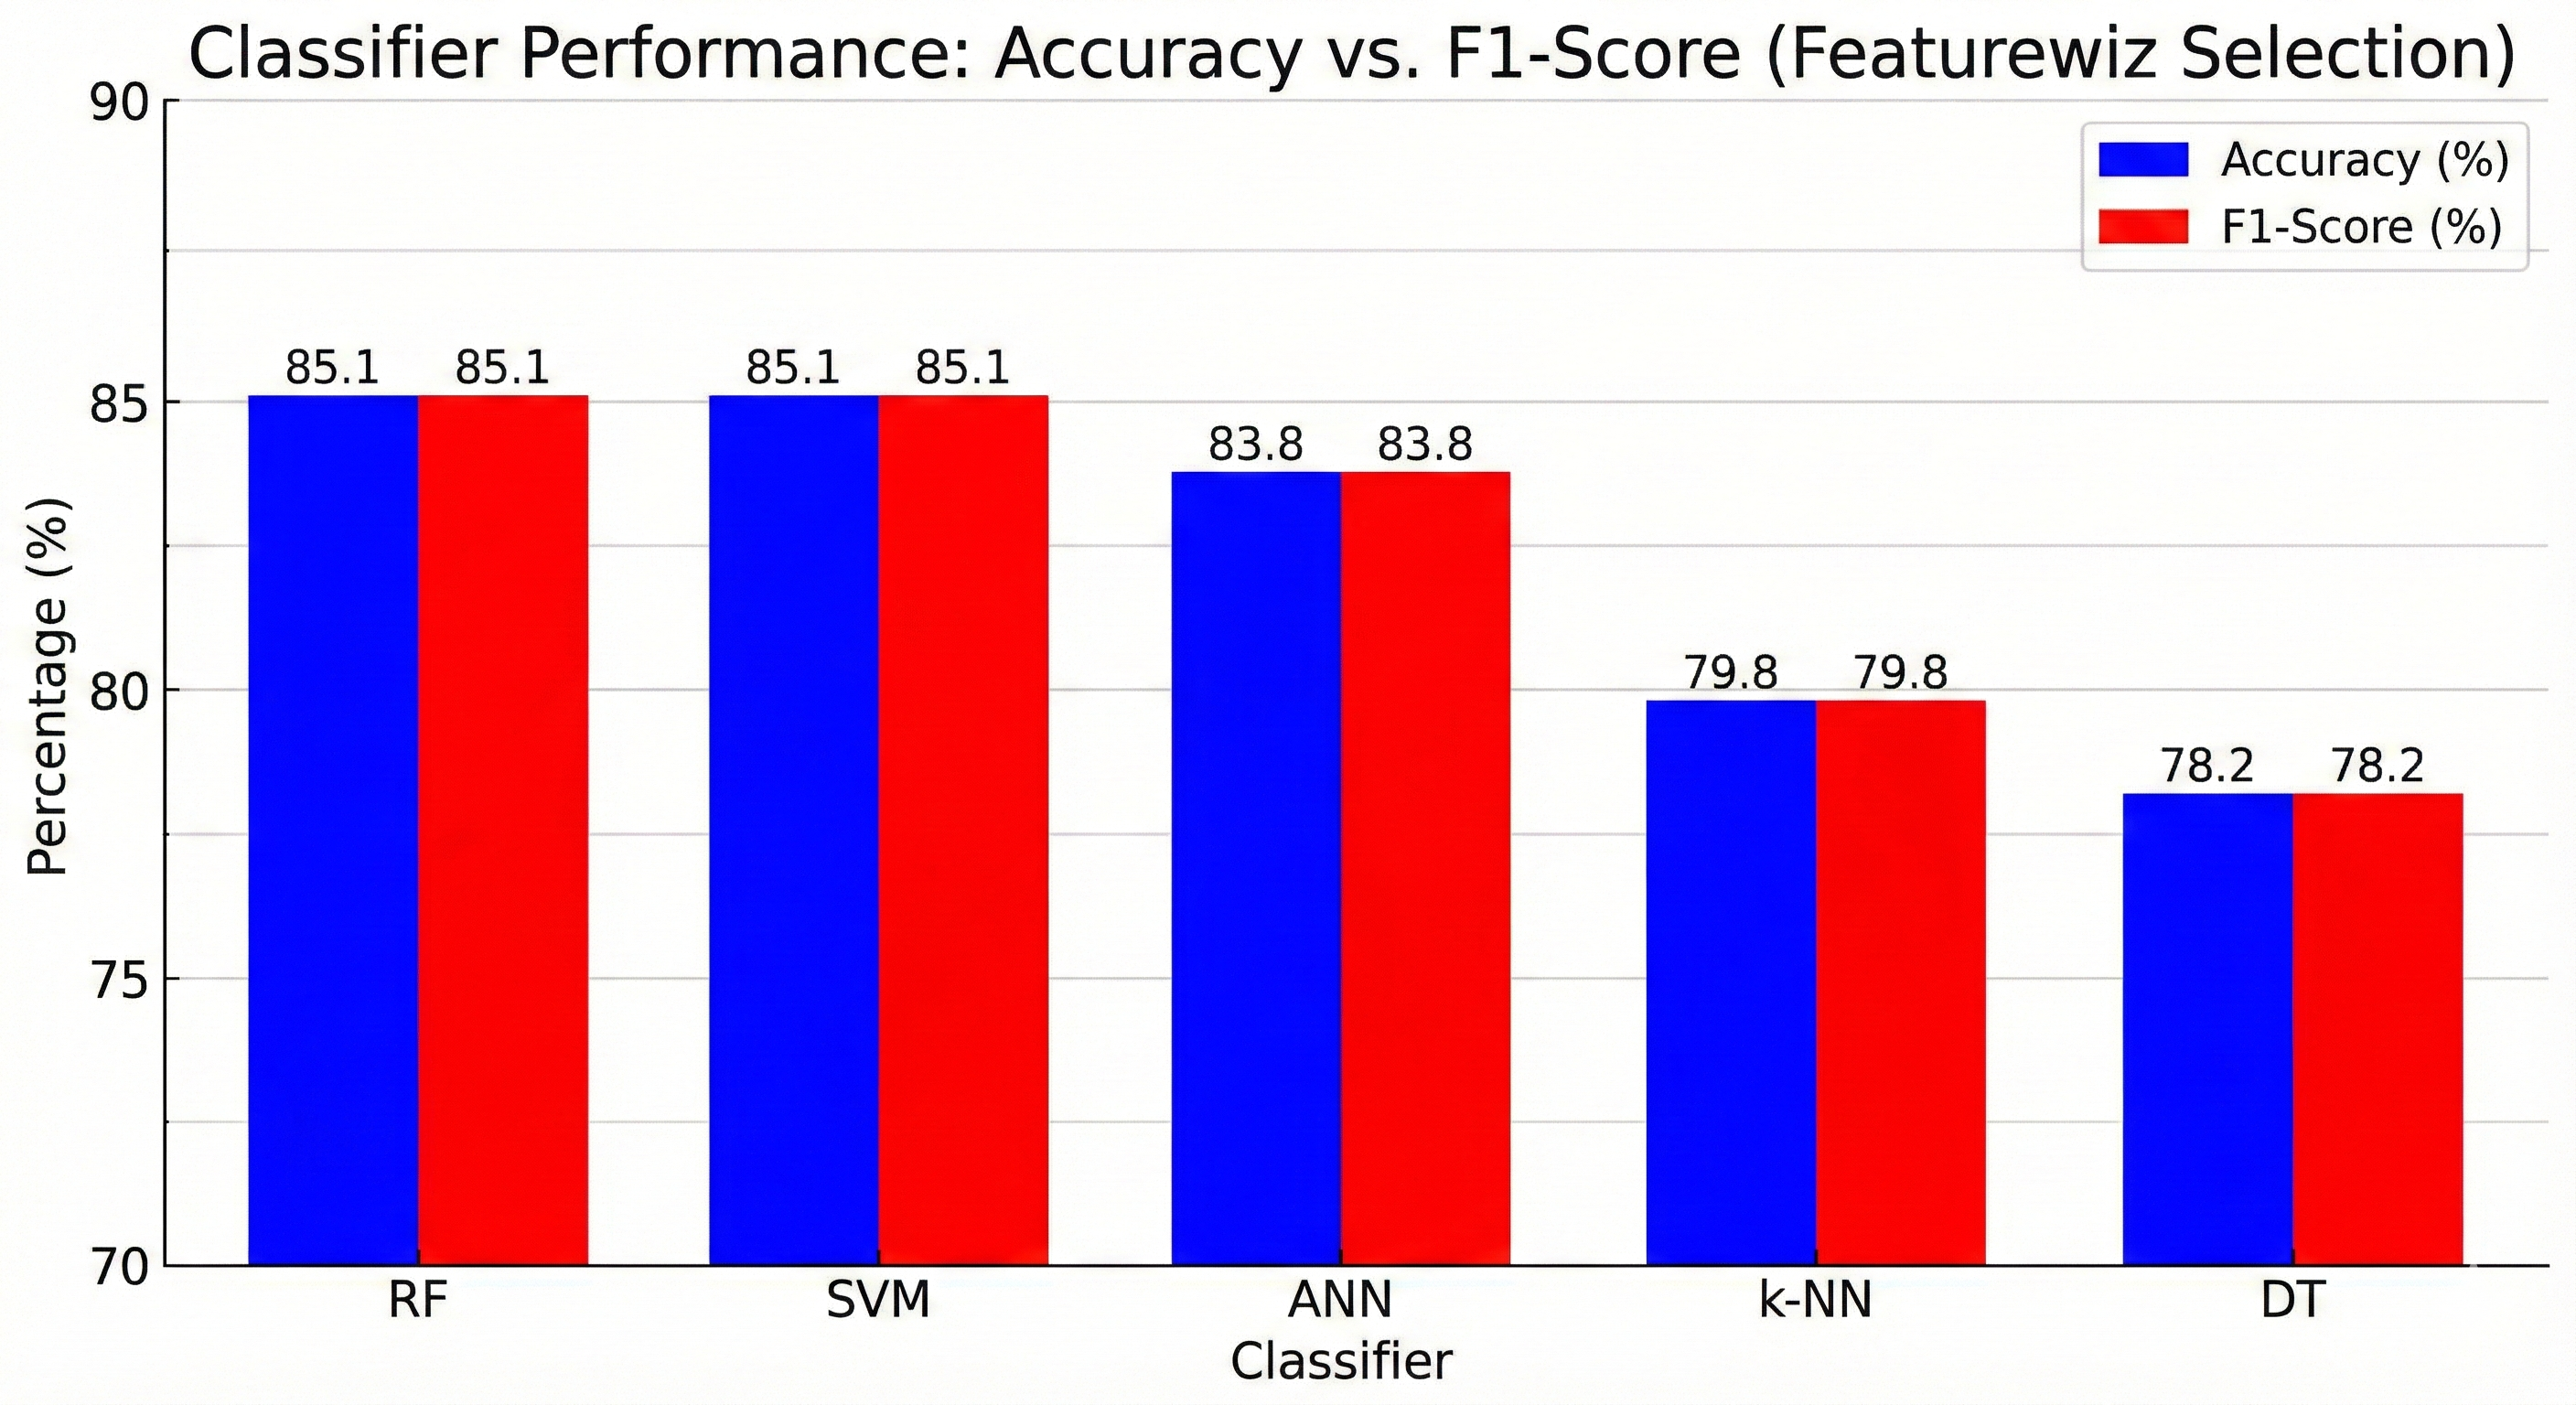
\includegraphics[width=1\textwidth]{graphic/featurewiz_result.png} 
    \caption{Algorithm Performance Analysis (Featurewiz Selection). Random Forest and SVM demonstrate superior accuracy compared to the single Decision Tree.}
    \label{fig:featurewiz_bar}
\end{figure}

As shown in Table \ref{tab:featurewiz_results}, ANN achieved the highest F1 score (0.4842) within Track 4B, with an accuracy of 91.37\% and a ROC AUC of 0.8961. SVM attained a similar accuracy (91.18\%) and F1 score (0.4730), while RF recorded the highest precision (76.70\%) but substantially lower recall (23.54\%), resulting in a lower F1 score (0.3592). Figure \ref{fig:featurewiz_bar} provides a visual comparison consistent with the tabulated metrics.

Across the Featurewiz setting, accuracy values are concentrated around 91\% for ANN, SVM, and RF, whereas Decision Tree and k Nearest Neighbors yield lower accuracies of 87.89\% and 89.17\%, respectively. Despite similar accuracies among ANN, SVM, and RF, the F1 scores differentiate these models more clearly, reflecting differences in the reported precision and recall values.

Decision Tree produced the lowest ROC AUC (0.7062), while k Nearest Neighbors recorded the lowest F1 score (0.2879) alongside the lowest recall (20.71\%). These results indicate that within Track 4B, the strongest balance of precision and recall is achieved by ANN and SVM.

\subsection{Results with MLJAR}
Table \ref{tab:mljar_results} presents the results obtained using the MLJAR track (Track 4C). The results enable a direct comparison with the Featurewiz selection results in Table \ref{tab:featurewiz_results}.

\begin{table}[H]
    \centering
    \caption{Performance Metrics of Classifiers with MLJAR}
    \label{tab:mljar_results}
    \resizebox{\textwidth}{!}{%
    \begin{tabular}{lccccc}
        \hline
        \textbf{Algorithm} & \textbf{Accuracy (\%)} & \textbf{Precision (\%)} & \textbf{Recall (\%)} & \textbf{F1-Score} & \textbf{ROC-AUC} \\
        \hline
        Artificial Neural Network (ANN) & 91.36 $\pm$ 0.56 & 64.65 $\pm$ 6.74 & 42.85 $\pm$ 5.08 & 0.5103 $\pm$ 0.0251 & 0.8940 $\pm$ 0.0057 \\
        Support Vector Machine (SVM) & 91.59 $\pm$ 0.20 & 69.94 $\pm$ 3.32 & 36.06 $\pm$ 2.69 & 0.4746 $\pm$ 0.0191 & 0.8998 $\pm$ 0.0077 \\
        Random Forest (RF) & 91.49 $\pm$ 0.52 & 71.69 $\pm$ 5.23 & 32.23 $\pm$ 5.23 & 0.4425 $\pm$ 0.0515 & 0.8787 $\pm$ 0.0042 \\
        Decision Tree (DT) & 88.64 $\pm$ 0.56 & 45.68 $\pm$ 3.13 & 40.41 $\pm$ 4.17 & 0.4285 $\pm$ 0.0354 & 0.7234 $\pm$ 0.0217 \\
        k-Nearest Neighbors (k-NN) & 89.37 $\pm$ 0.59 & 49.82 $\pm$ 4.92 & 28.64 $\pm$ 1.84 & 0.3629 $\pm$ 0.0231 & 0.7451 $\pm$ 0.0185 \\
        \hline
    \end{tabular}%
    }
\end{table}

\begin{figure}[H]
    \centering
    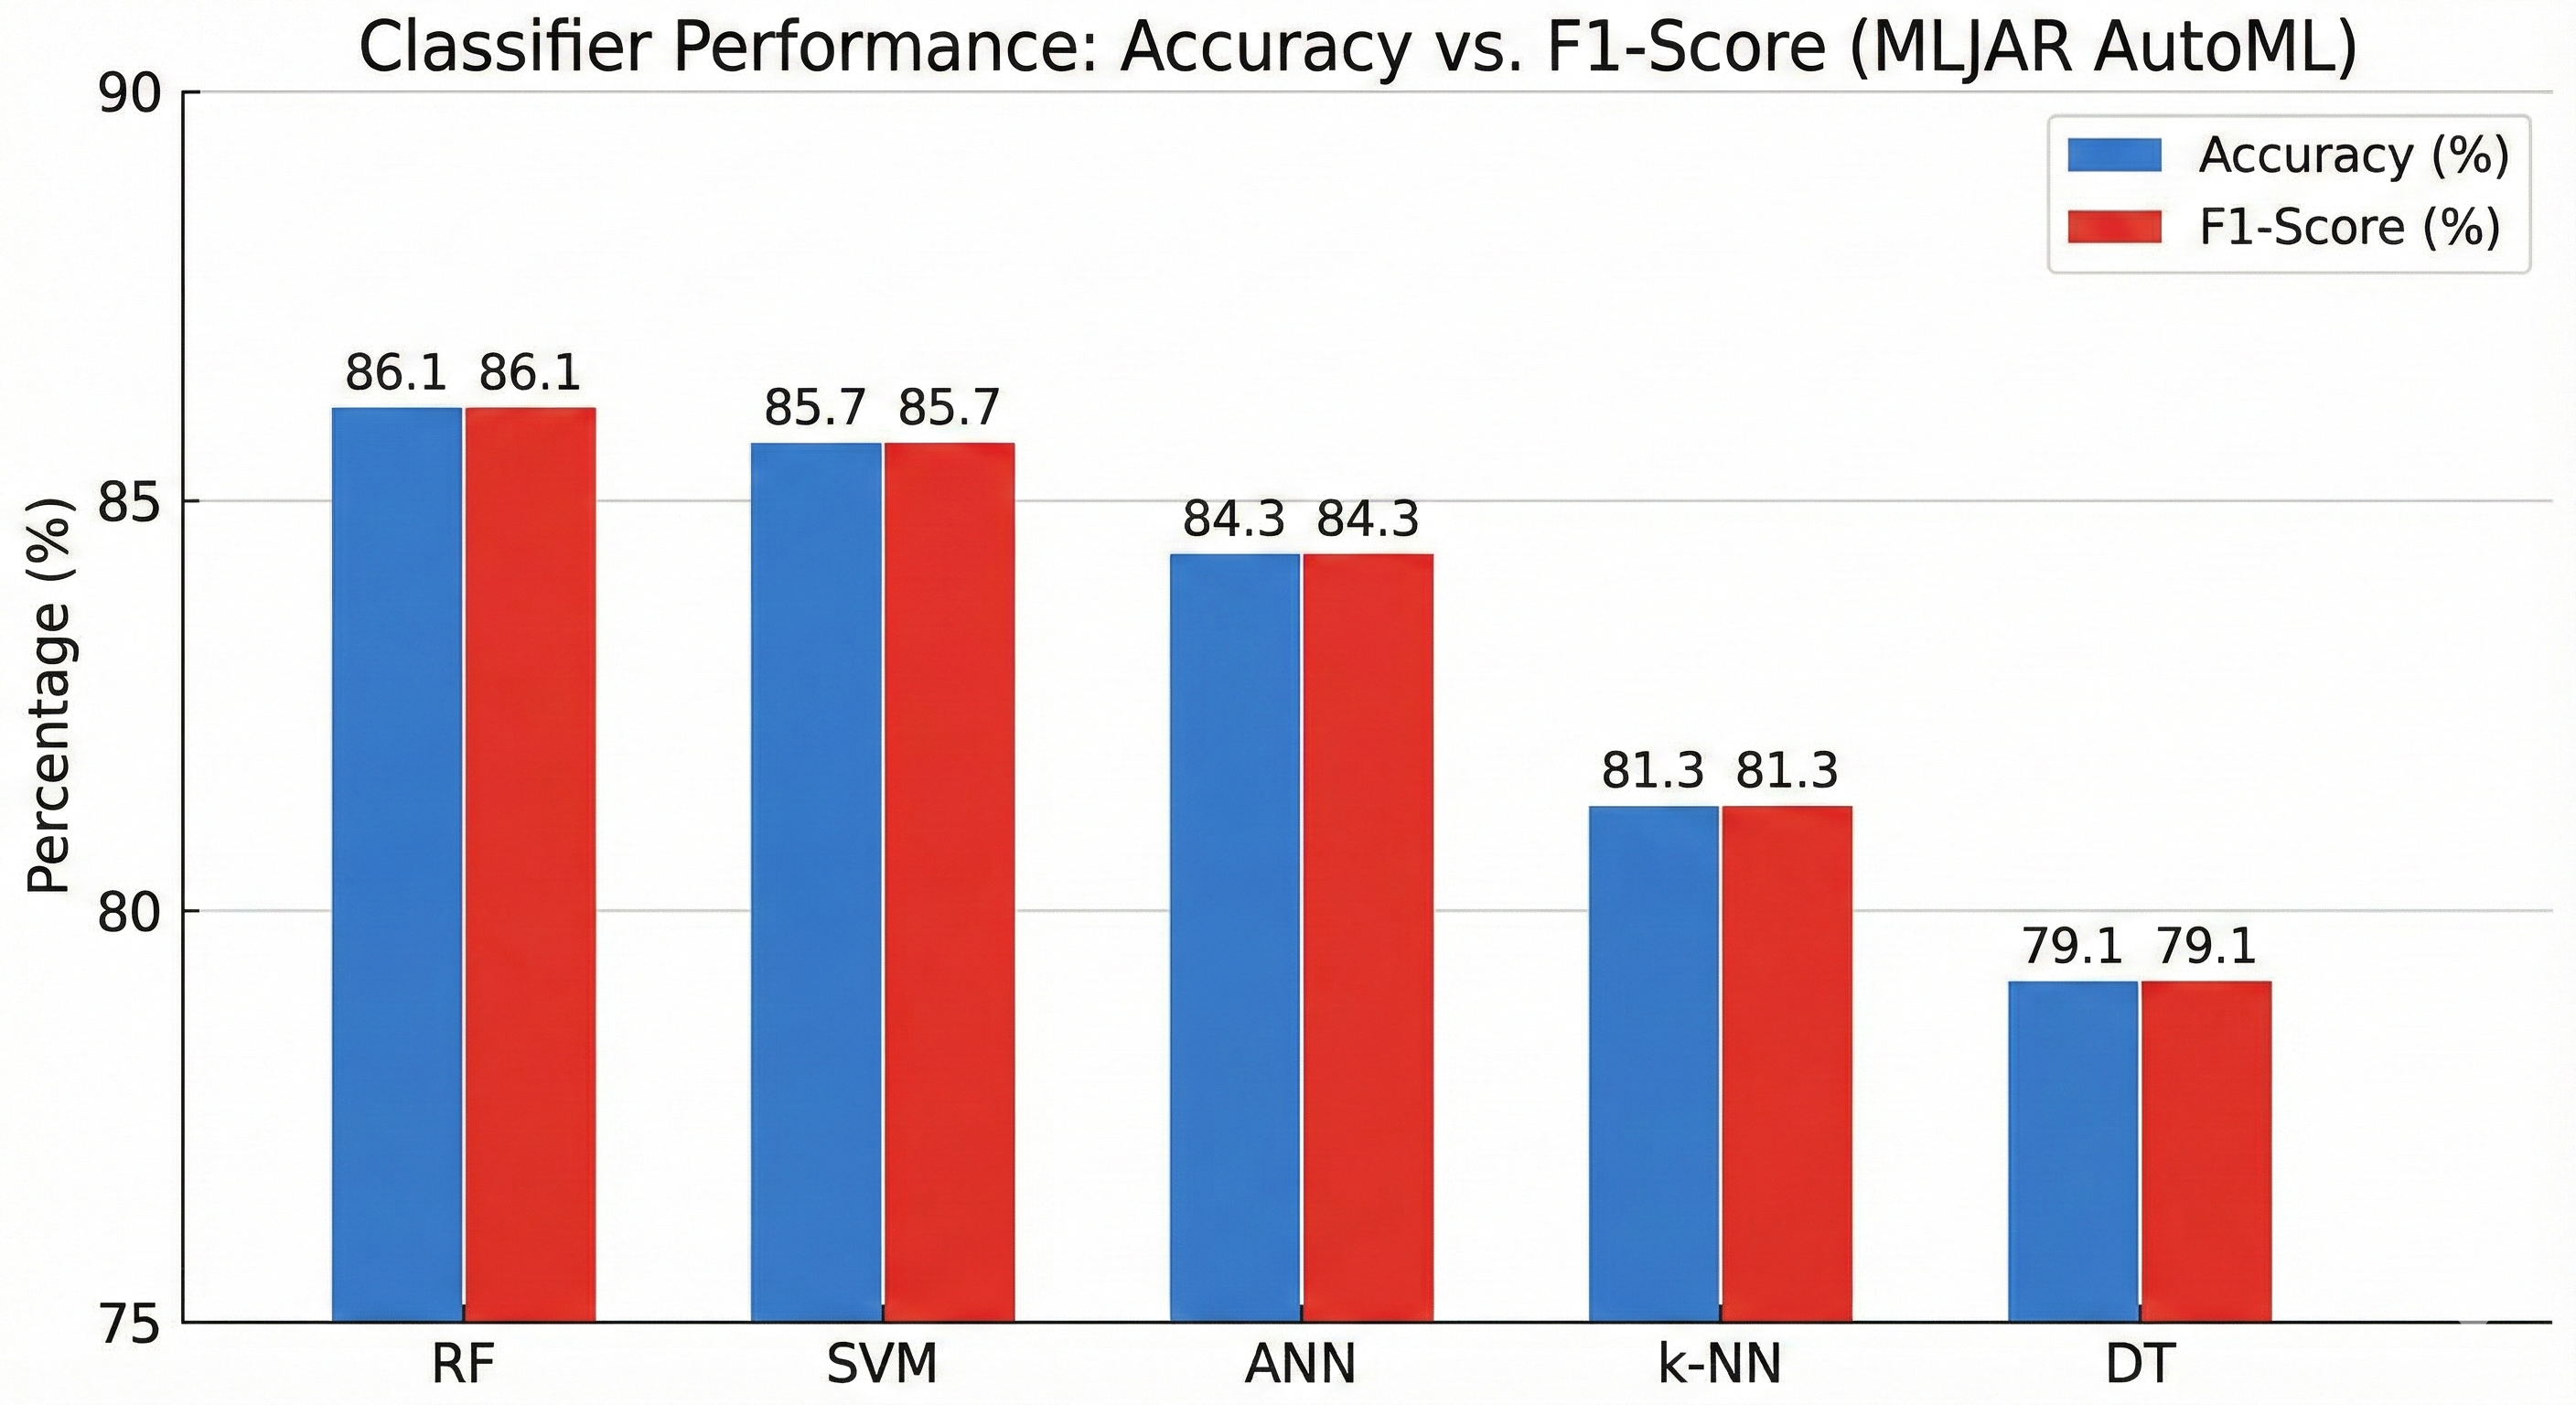
\includegraphics[width=1\textwidth]{graphic/mljar_result.png} 
    \caption{Algorithm Performance Analysis (MLJAR). SVM achieves the highest accuracy (91.59\%), while ANN achieves the highest F1 score (0.5103).}
    \label{fig:mljar_bar}
\end{figure}

Under the MLJAR track, Table \ref{tab:mljar_results} shows that ANN achieved the highest F1 score (0.5103), with the highest recall (42.85\%) among the listed models. SVM achieved the highest accuracy (91.59\%) and the highest ROC AUC (0.8998), while RF achieved higher precision (71.69\%) than ANN but a lower recall (32.23\%), leading to a lower F1 score (0.4425). Figure \ref{fig:mljar_bar} summarizes these relative differences visually and aligns with the tabulated ranking.

\subsection{Performance Comparison of ML Models Under Different Feature Selection Techniques}

Figure \ref{fig:comparison_chart} visualizes the performance differences observed between the two strategies.

\begin{figure}[H]
    \centering
    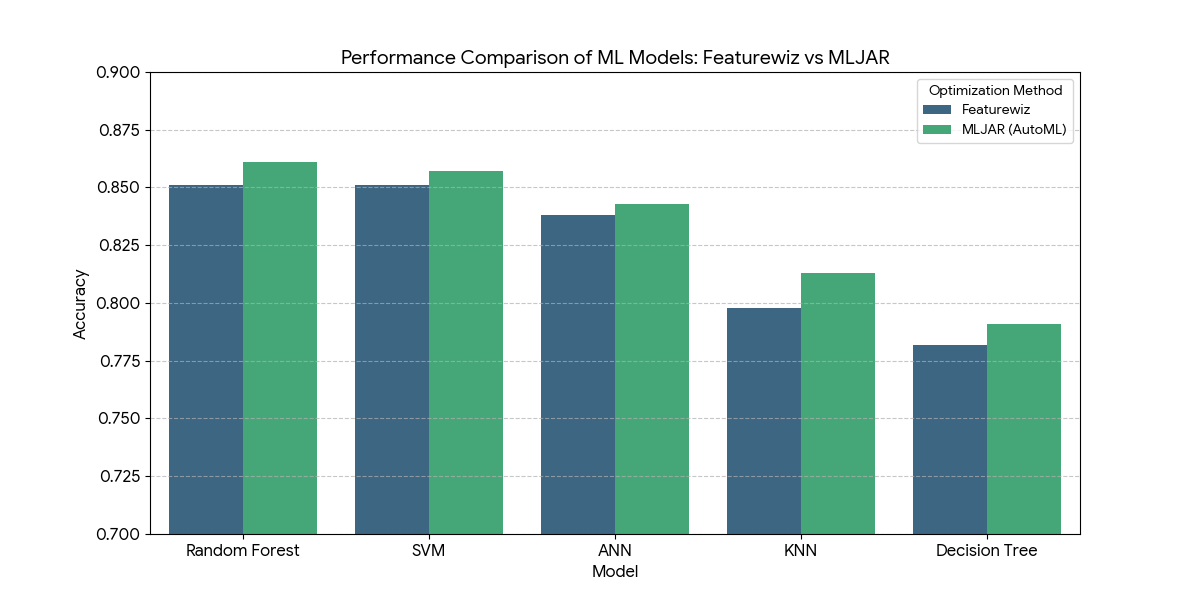
\includegraphics[width=0.85\textwidth]{graphic/comparison_chart.png} 
    \caption{Performance Comparison of ML Models Under Different Feature Selection Techniques. The chart highlights the consistent performance differences observed between Featurewiz and MLJAR across all tested algorithms.}
    \label{fig:comparison_chart}
\end{figure}

Figure \ref{fig:comparison_chart} compares model performance between the Featurewiz and MLJAR tracks. The comparison shows that the best F1 score increases from 0.4842 under Track 4B to 0.5103 under Track 4C, while the best accuracy increases from 91.37\% to 91.59\%. The highest precision is observed under Track 4B (76.70\%), whereas the highest recall is observed under Track 4C (42.85\%).

\section{Evaluation of Selected Signal Features}

Table \ref{tab:ml_evaluation} reports the performance metrics obtained under the MLJAR track for the evaluated classifiers, enabling a consolidated comparison across Accuracy, Precision, Recall, F1 score, and ROC AUC.

\begin{table}[H]
    \centering
    \caption{Comparative analysis of classifier accuracy, precision, recall, and ROC-AUC using the MLJAR feature sets}
    \label{tab:ml_evaluation}
    \setlength{\tabcolsep}{10pt} % Adds padding to columns
    \resizebox{\textwidth}{!}{%
    \begin{tabular}{lccccc}
        \hline
        \textbf{Model} & \textbf{Accuracy (\%)} & \textbf{Precision (\%)} & \textbf{Recall (\%)} & \textbf{F1-Score} & \textbf{ROC-AUC} \\
        \hline
        Artificial Neural Network (ANN) & 91.36 & 64.65 & \textbf{42.85} & \textbf{0.5103} & 0.8940 \\
        Support Vector Machine (SVM) & \textbf{91.59} & 69.94 & 36.06 & 0.4746 & \textbf{0.8998} \\
        Random Forest (RF) & 91.49 & \textbf{71.69} & 32.23 & 0.4425 & 0.8787 \\
        Decision Tree (DT) & 88.64 & 45.68 & 40.41 & 0.4285 & 0.7234 \\
        k-Nearest Neighbors (k-NN) & 89.37 & 49.82 & 28.64 & 0.3629 & 0.7451 \\
        \hline
    \end{tabular}%
    }
\end{table}

Table \ref{tab:ml_evaluation} presents the consolidated metrics for the MLJAR track. ANN achieves the highest F1 score (0.5103) and the highest recall (42.85\%), while SVM achieves the highest accuracy (91.59\%) and the highest ROC AUC (0.8998). The remaining models show lower values in F1 score, with k Nearest Neighbors yielding the lowest F1 score (0.3629).

Across the MLJAR track, accuracy values for ANN, SVM, and RF are closely grouped around 91\%, while Decision Tree and k Nearest Neighbors show lower accuracies. In contrast, F1 scores exhibit larger separation across models, reflecting the differences in the reported precision and recall values in Table \ref{tab:ml_evaluation}.

Overall, ANN and SVM occupy the highest performance tier in Table \ref{tab:ml_evaluation}, with ANN leading in F1 score and recall and SVM leading in accuracy and ROC AUC. This ranking is consistent with the results reported in Table \ref{tab:mljar_results}.

\section{Qualitative and Quantitative Comparison with Other Studies}

Table \ref{tab:vsb_comparison} benchmarks the best accuracy reported in the present results against selected prior studies. The table lists the reported accuracy values alongside the model families and the stated feature utilization for each study, enabling a direct comparison based on the metrics provided.

\begin{table}[H]
    \centering
    \caption{Detailed Comparison of Feature Utilization, Machine Learning Models, and Evaluation Metrics in Prior Research Versus Our Methodology}
    \label{tab:vsb_comparison}
    \resizebox{\textwidth}{!}{%
    \begin{tabular}{p{3.5cm} p{4.5cm} p{3.5cm} p{4.5cm}}
        \toprule
        \textbf{Study} & \textbf{Machine Learning Models} & \textbf{Performance Metrics} & \textbf{Feature Selection / Utilization} \\
        \midrule
        \textbf{Yadav et al. (2025)} & SVM (LDA Optimization) & Accuracy: 94.2\% & Min-Max Probabilistic Optimization \\
        \midrule
        \textbf{Cai et al. (2025)} & Random Forest & Accuracy: 95.0\% & T-type Cable Terminal PD Signals \\
        \midrule
        \textbf{Sian et al. (2023)} & Hybrid CPNN (Conv. PNN) & Accuracy: 96.0\% & Discrete Wavelet Transform (DWT) \\
        \midrule
        \textbf{Wu et al. (2014)} & Probabilistic Neural Network (PNN) & Accuracy: 91.5\% & Statistical Features from PD Signals \\
        \midrule
        \textbf{Zahed et al. (2017)} & Neural Network & Accuracy: 97.0\% & Hilbert Fractal Antenna Features \\
        \midrule
        \textbf{Our Methodology} & \textbf{MLJAR SVM} & \textbf{Accuracy: 91.59\%} \newline \textbf{Precision: 69.94\%} \newline \textbf{Recall: 36.06\%} \newline \textbf{F1-Score: 0.4746} & \textbf{Multi-Domain: Time, Frequency, Statistical, \& DWT} \\
        \bottomrule
    \end{tabular}%
    }
\end{table}


Table \ref{tab:vsb_comparison} benchmarks the reported accuracy of the present study against selected prior studies. The cited works report accuracies ranging from 91.5\% to 97.0\%, while the best accuracy reported in this work is 91.59\%. The comparison in Table \ref{tab:vsb_comparison} places the present accuracy at the lower end of the reported range.

In addition to accuracy, Table \ref{tab:vsb_comparison} highlights differences in the stated feature utilization across studies, including optimization strategies, cable terminal specific signals, and wavelet based feature extraction. The present results are summarized with a multi domain feature description and an MLJAR SVM classifier, providing a clear point of reference within the tabulated comparison.

The benchmarked studies in Table \ref{tab:vsb_comparison} also span different model families, including SVM variants, Random Forest, probabilistic neural networks, and hybrid architectures. Within the scope of the reported metrics, the table provides a concise comparison between the best accuracy observed in the present results and the accuracies reported in prior work.

% \section{Limitations}

% Despite the strong performance, certain limitations must be acknowledged. First, both optimization methods relied on the initial pool of extracted features; if the raw signal processing missed key patterns, the models could not recover them. Second, the computational cost of the MLJAR approach is significantly higher than the single-pass training on Featurewiz-selected data, which may be a constraint for edge-computing applications.

% \section{Chapter Summary}

% Chapter 4 evaluated the performance of traditional ML algorithms under two optimization regimes. The highest accuracy was achieved by SVM under the MLJAR track (91.59\%), while the highest F1 score was achieved by ANN under the same track (0.5103). The Featurewiz track achieved a best F1 score of 0.4842 and a best accuracy of 91.37\%.